\documentclass[tikz,border=2pt]{standalone}
\usepackage{amsmath,amssymb}
\usepackage{tikz}
\usetikzlibrary{arrows.meta}

\begin{document}
% Two linear equations in two unknowns are two lines; solving the system means finding the
% points common to both.
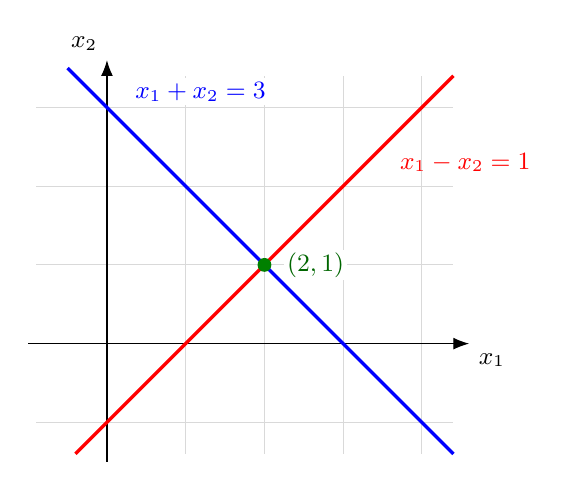
\begin{tikzpicture}[every node/.style={font=\small}, >={Latex[length=2mm]}]
	\draw[gray!30, step=1] (-0.9,-1.4) grid (4.4,3.4);
	\draw[->] (-1,0) -- (4.6,0) node[below right] {$x_1$};
	\draw[->] (0,-1.5) -- (0,3.6) node[above left] {$x_2$};
	\draw[blue, very thick] (-0.5,3.5) -- (4.4,-1.4);
	\node[blue, anchor=west, fill=white, inner sep=1.5pt] at (0.3,3.2) {$x_1+x_2=3$};
	\draw[red, very thick] (-0.4,-1.4) -- (4.4,3.4);
	\node[red, anchor=west] at (3.6,2.3) {$x_1-x_2=1$};
	\fill[green!50!black] (2,1) circle (2.5pt) node[right=7pt, inner sep=1pt, fill=white, text=green!40!black] {$(2,1)$};
\end{tikzpicture}
\end{document}
